\documentclass[smaller,professionalfonts,15pt]{beamer}
\usepackage{fontspec,unicode-math}
\usepackage{lipsum, lmodern}
\usepackage{polyglossia}
\usepackage{bncc}
\usepackage[livrosdecriacao]{logoedlab}
\setdefaultlanguage{brazilian}

\usetheme[widescreen]{PraterStreet} % or Median, or Metro, or PraterStreet, or Milano
\setromanfont{Avenir Next Condensed}
\setsansfont{Avenir Next Condensed}
\setmonofont[Color={0019D4}]{Avenir Next Condensed}

\author{Crônicas e contos}
\title{Lima Barreto}
\institute{Pázmány Péter Catholic University}
\date{\today}

\begin{document}

\definecolor{studiointro}{rgb}{0, 0, 0}
\setbeamercolor{block title}{bg=studiointro,fg=black}


\begin{frame}
\begin{raggedleft}
\Huge Crônicas e contos\\
\huge Lima Barreto\\\bigskip
\normalsize
Tema: Ficção, mistério e fantasia\\	
Gênero: Conto, crônica e novela\\
\end{raggedleft}

%\vspace{2cm}\includegraphics[width=4cm]{\logoeditora}
\end{frame}

\begin{frame}
\begin{figure}
\hfill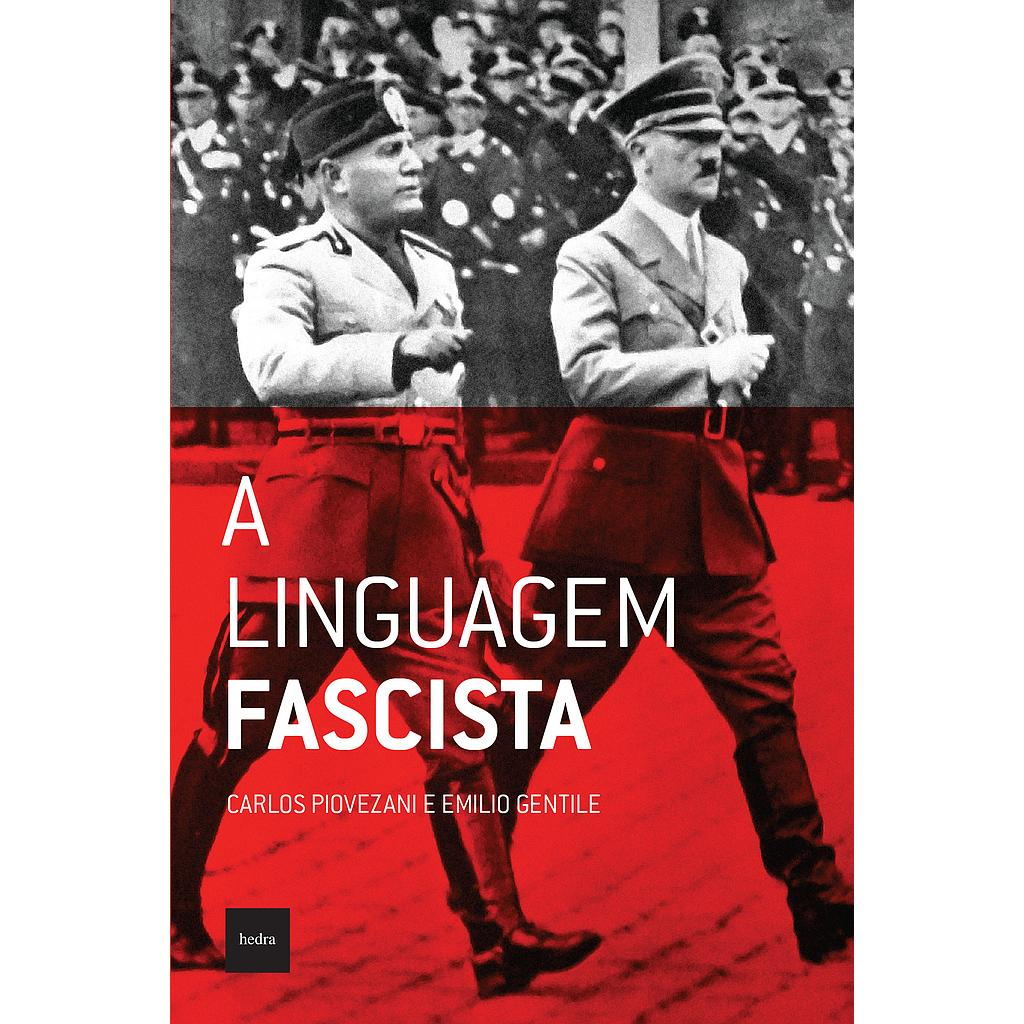
\includegraphics[width=6cm]{cover.jpeg}
\end{figure}
\end{frame}


\begin{frame}[plain]{Habilidades (BNCC)}
\vspace{-2cm}
\BNCC{EM13LGG101}
\BNCC{EM13LGG201}
\BNCC{EM13LGG301}
\BNCC{EM13LP33}
\BNCC{EM13LP45}
\BNCC{EM14LP48}
\BNCC{EM13LP50}
\BNCC{EM13LP53}
\BNCC{EM13CHS101}
\BNCC{EM13CHS102}
\BNCC{EM13CHS503}
\BNCC{EM13CHS504}
\BNCC{EM13CHS601}
\end{frame}

\end{document}
